\section{Angular Measurements}
\makelabheader %space for name & lab partner

In astronomy, we often talk about the ``angular size'' of an object.
This is just a way of expressing how big the object appears to be, or
in other words how much of our field of view it takes up.  For
instance, in the picture below (which is the same as the picture in
your previous lab), the two objects have the same angular size,
because they ``fill up'' the same angle in the observer's
field of view.

\medskip
%\centerline{\epsfxsize 6in\epsfbox{localdistance/localdistance1.eps}}
\centerline{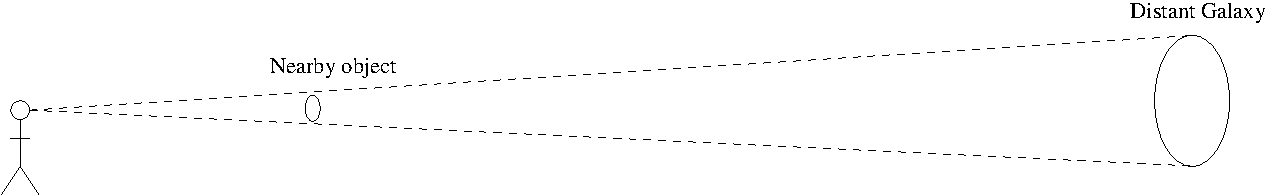
\includegraphics[width=\textwidth]{localdistance/localdistance1.pdf}}
\medskip

The angular size is related to the actual size of the object and the
object's distance.  That relationship is going to be extremely useful
to us, so I want you to spend a little while right now working it out.

Here's a picture of an object.  The angular size is the angle $\alpha$
on the left.  The distance from the observer to the object is $d$, and
the actual size of the object is $s$.  Our goal is to relate the
three numbers $\alpha,s,d$.

\medskip
%\centerline{\epsfbox{angularsize/angularsizefig1.eps}}
\centerline{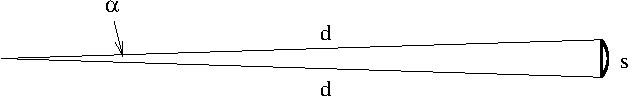
\includegraphics[width=4in]{angularsize/angularsizefig1.pdf}}
\medskip

(Note: Your textbook uses the symbol $D$ instead of $s$ for
the size of the object.  I don't like that, because I think it's
too easy to mix up $d$ and $D$, so I'm going to call it $s$ instead.)

We can use trigonometry to relate these three numbers, but the
mathematics is a bit annoying.  Fortunately, as long as the angle
$\alpha$ is very small (which it almost always is
in astronomical observations), there is a simplified
relationship between these numbers that doesn't involve
any trig.  Here's how it works.

In the picture below, the straight line on the right
represents the
object.  The length of this line is the exact value of $s$, the object's
size.  The picture also shows a curved line.  That curve is an arc
of a circle centered on the observer.  Because it's curved and not straight,
the length of this arc is not quite the same as $s$.  On the other hand,
if the angle $\alpha$ is very small, then this curve is almost the same
length as the straight line.  For this reason, {\it we are going to allow
ourselves to pretend that the length of that curved arc is the
same as $s$.}  To figure out the length of the straight line, we'd
need trig, but we can figure out the length of the arc with just
geometry.


\medskip
%{\epsfbox{angularsize/angularsizefig2.eps}}
\centerline{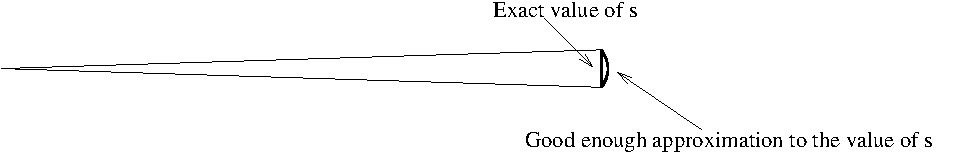
\includegraphics[width=6in]{angularsize/angularsizefig2.pdf}}
\medskip

\pagebreak[4]
Here's yet another picture of the situation.  Now the observer is at
the center.  The solid arc represents the size of the object being observed,
and $d$ is the distance from observer to object.  The dashed circle
is an imaginary circle centered on the observer.

\medskip
%\centerline{\epsfxsize 2.5in\epsfbox{angularsize/angularsizefig3.eps}}
\centerline{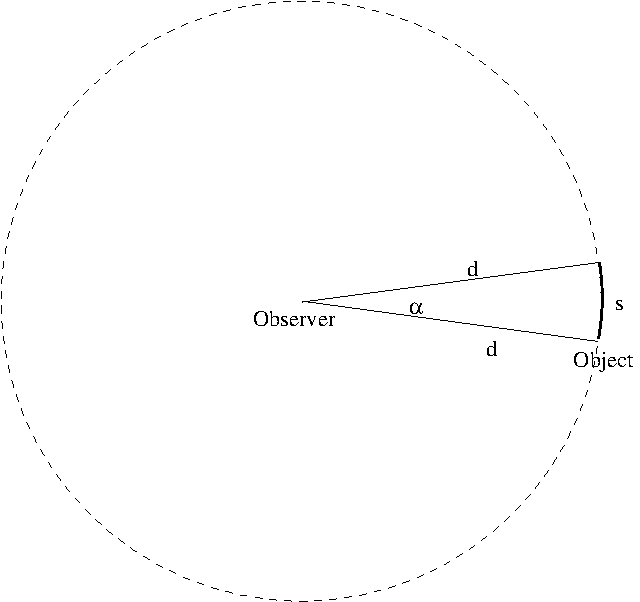
\includegraphics[width=3.5in]{angularsize/angularsizefig3.pdf}}
\medskip

Well, let's get started.



1. Suppose that the angle $\alpha$ is one degree.  What fraction
of the whole circle is covered by the arc $s$?

\answerspace{1in}

2. Remember that the circumference of a circle is $2\pi$ times the
radius.  What is the length of the arc $s$, in terms of the distance
$d$?  Continue to assume that $\alpha$ is one degree.
(Your answer here should say $s=$ something times $d$.)


\answerspace{1in}


Repeat steps 1 and 2, but this time assume that $\alpha=2^\circ$.


\answerspace{1.5in}

\pagebreak[2]
Repeat steps 1 and 2, but this time don't assume any particular
value for $\alpha$.  Instead, your answers will be algebraic
expressions including $\alpha$ as an unknown variable.
Your final result should say $s=$ something involving both $\alpha$ and $d$.


\answerspace{2in}

Once you've got this expression worked out, show it to me.  This
extremely useful fact is known as the ``small-angle formula.''

Now that you know the small-angle formula, what do you use it for?
The main thing is that any time you know two of the numbers $\alpha,s,d$,
you can use the formula to get the third one.  Try these out:

The Moon is 3476 kilometers in diameter, and it's 380\,000 kilometers
away.  What is the angular size of the Moon?

\answerspace{1in}

The Sun's angular size is 0.53 degrees, and the Sun is 150 million
kilometers away.  What's the Sun's diameter in kilometers?

\answerspace{1in}

\pagebreak[3]
Most of the time, angles in astronomy are much smaller even than one degree.
For this reason, astronomers usually measure angles in units called
{\it arc-minutes} and {\it arc-seconds}.  One arc-minute is one-sixtieth
of a degree:
$$
1' = \left(\frac{1}{60}\right)^\circ.
$$
($'$ means ``minute''; $^\circ$ means ``degree.'')
One arc-second is one-sixtieth of a minute:
$$
1''=\left(\frac{1}{60}\right)'.
$$
($''$ means ``second.'')

How many arc-seconds are in one degree?

\answerspace{1in}

A decent astronomical telescope can see things whose angular size is
as small as $1''$.  How far away would your lab partner have to be in
order for the angular distance between their eyes to be equal to
$1''$?  You'll have to measure the distance between your partner's
eyes to answer this.  (If your partner is any further away than this,
then the telescope would no longer be able to see your partner's eyes
as two separate objects; they'd be blurred into one blob.)


\answerspace{1in}

Optional question:
If you know and remember your trig and feel like it, try answering
the last question using trig instead of the small-angle formula.  Does
it make a significant difference in the final result?

